%% Version: 0.2 (31.01.2018)

%% Choose language: english or german
%% Choose Thesis type: seminar, bachelor, master, techreport
%% Use 'declaration' parameter if you want to generate declaration page
%% Use 'final' to disable Todo-notes from final version without deleting each one of them
\documentclass[german,seminar]{KITthesis}

%% ---------------------------------
%% | Information about the thesis  |
%% ---------------------------------
\title{\Huge Hybrider OP-Saal}
\titleotherlanguage{Hybrid Operating Room}

\author{Theresa Heine}
\address{Brauerstraße 19}
\city{76137 Karlsruhe}
\email{uuecn@student.kit.edu}

\keywords{Hybrider OP-Saal, Netzwerkkommunikation, Datenaustausch, Herausforderungen}
\keywordsotherlanguge{Hybrid Operating Room, Network Communication, Data Exchange, Challenges}

%% Study program or a seminar/subject
\studyprogram{\LARGE Informatik in der Medizin}

%% Name of your institute (Default: IAR-IPR)
% \institute{}
%% Name of your faculty (Default: KIT-Fakultät für Informatik
% \KITfaculty{}
%% Address of your institute (Default: Engler-Bunte-Ring 8)
% \instituteaddress{}
%% Insitute City (Default: 76131 Karlsruhe)
% \institutecity{}

\reviewerone{Prof. Dr.-Ing. Torsten Kröger}
\reviewertwo{Prof. Dr.-Ing. habil. Björn Hein}
%
% %% The advisors are PhDs or Postdocs
\advisorone{M.Sc. Christian Marzi}
% %% The second advisor can be omitted
\advisortwo{M.Sc. D}
%
% %% Please enter the start end end time of your thesis
\editingtime{16. April 2018}{18. Juni 2018}

%% --------------------------------
%% | Settings for word separation |
%% --------------------------------
% Help for separation:
% In german package the following hints are additionally available:
% "- = Additional separation
% "| = Suppress ligation and possible separation (e.g. Schaf"|fell)
% "~ = Hyphenation without separation (e.g. bergauf und "~ab)
% "= = Hyphenation with separation before and after
% "" = Separation without a hyphenation (e.g. und/""oder)

% Describe separation hints here:
\hyphenation{
% Pro-to-koll-in-stan-zen
% Ma-na-ge-ment  Netz-werk-ele-men-ten
% Netz-werk Netz-werk-re-ser-vie-rung
% Netz-werk-adap-ter Fein-ju-stier-ung
% Da-ten-strom-spe-zi-fi-ka-tion Pa-ket-rumpf
% Kon-troll-in-stanz
}

\usepackage{graphicx}
\usepackage[format=plain, indention=0cm]{caption}
\usepackage{babel,blindtext}


\settitle
%%%%%%%%%%%%%%%%%%%%%%%%%%%%%%%%%
%% Here, main documents begins %%
%%%%%%%%%%%%%%%%%%%%%%%%%%%%%%%%%
\begin{document}

%% Set PDF metadata
\setpdf

%% Title Page
\includetitle

\includedeclaration

\includeacknowledgments

%% ----------------
%% |   Abstract   |
%% ----------------
%% An abstract both in English
%% and German is mandatory.
%%
%% The text is included from the following files:
%% - Content/0-Abstract_EN
%% - Content/0-Abstract_DE
\includeabstract

\inculdetableofcontents

\makenomenclature

\setmainpart

\chapter{\iflanguage{ngerman}{Übersicht Hybrider OP-Saal}{Overview}}
\label{sec:overview}

\subsection{Hybrider OP-Saal vs. Standard OP-Saal / Stand der Technik}
1. Der digitale Operationssaal- Kapitel 2
	"Die Anforderungen an einen Operationssaal sind in den vergangenen fünf Jahren
	deutlich gestiegen. Das gilt besonders für alle spezialchirurgischen Fächer mit minimal-
	invasiven Zugängen und endoskopischer Visualisierung wie z. B. der HNO-Chirurgie
	(Abb. 2.1). Neue Funktionen wie Instrumentennavigation, Kollisionswarnung,
	Neuromonitoring, intraoperativer Ultraschall, Messsysteme, Mikromanipulatoren,
	Telekonferenzen, kontinuierliche Aufzeichnungen des Eingriffs, Einblick in die Elektronische
	Patientenakte (EPR) und das radiologische Archiv (S-PACS) erweitern die
	Möglichkeiten eines OP-Saals drastisch."
	
	"Die derzeit verfügbaren Operationssäle werden meist in konventionelle und integrierte
	OP-Säle unterteilt (z. B. OR1 der Karl Storz GmbH und Co. KG; Endoalpha der
	Olympus Deutschland GmbH; iSuite der Stryker GmbH und Co. KG) [1–3]. Die Definition
	des „integrierten OP-Saals“ ist dabei jedoch unscharf. Häufig wird bereits die Realisierung
	minimaler Veränderungen wie RGB-Licht in den Wänden oder eine versteckte
	Kabelführung mit diesem Begriff beworben. Diese OP-Säle umfassen vor allem eine
	Verbesserung der architektonischen sowie räumlichen und nur teilweise der funktionellen
	Integration.
	Weiterführende Integrationslösungen verfügen heute über einen proprietären
	Datenbus zur Vernetzung ausgewählter Komponenten [4, 5]. Durch einen solchen
	Bus ist die zentrale Bedienung von Medizingeräten über ein gemeinsames Interface
	möglich. Besonders diese Vorarbeiten sind heute die Voraussetzungen für die nächste
	Generation von OP-Systemen."

2. http://www.ctsnet.org/article/cardiovascular-hybrid-or-clinical-technical-considerations	30.04.18 16:15
	"Mobile C-arms, ultrasound, and endoscopy are standard of care for many operations. However, complex transcatheter techniques demand high powered equipment to visualize thin guide wires, quantify small vessel diameters, and evaluate delicate anastomoses. Because of their size and complexity these integrated endovascular suites or Hybrid ORs require special considerations, planning, and design as well as new skills to be learned by the team."

3. http://www.innovations-report.de//html/berichte/medizin-gesundheit/saarlaendische-shg-kliniken-setzen-hybrid-op-201121.html 30.04.18 15:45	
	"Ein Hybrid-Operationssaal ist die Kombination aus hochsterilem Operationssaal und Systemen zur intraoperativen Bildgebung wie Computertomografen oder Angiografieanlagen. Dadurch ist es möglich, Diagnostik, interventionelle und/oder operative Therapie und Therapiekontrolle in einer Sitzung vorzunehmen.
	Der Betrieb von Hybrid-Operationssälen ermöglicht weniger invasive Behandlungsverfahren. Gleichzeitig wird das Zusammenarbeiten verschiedener Fachdisziplinen vorangebracht, was zur qualitativen Verbesserung der Behandlungen führt. Die häufigsten Anwendungen finden sich bisher in der Kardiologie und Herzchirurgie (minimalinvasive Implantationen von Herzklappen) sowie in der Gefäßchirurgie."
	
4. http://www.innovations-report.de/html/berichte/medizintechnik/dresdner-uniklinikum-nimmt-high-end-hybrid-op-in-betrieb.html 30.04.18 16:00
	"Der Begriff „Hybrid-OP“ steht für einen modernen Operationssaal der mit Geräten medizinischer Bildgebung kombiniert wird. In einem solchen Saal lassen sich beispielsweise auch bei offenen OP Röntgenbilder anfertigen und Interventionen mit Kathetern vornehmen."

5. Der digitale Operationssaal- Kapitel 3
	"Die Austauschbarkeit
	von einzelnen Medizinprodukten ist beschränkt. Eine Integration von Drittanbieterkomponenten
	kann nur in Kooperation mit dem Hersteller des Integrationssystems
	erfolgen [5]. Als wesentlicher Grund für den Einsatz von monolithischen Lösungen
	werden von Herstellern die Notwendigkeit der Konformitätsbewertung von Medizinprodukten
	sowie die in diesem Zusammenhang entstehende Problematik des Risikomanagements
	vernetzter Medizinprodukte angeführt."
\subsection{Geräte und System im Hybriden OP-Saal}
1. https://www.revolvy.com/main/index.php?s=Hybrid%20operating%20room&item_type=topic 01.05.18 18:00
	"A hybrid operating room is a surgical theatre that is equipped with advanced medical imaging devices such as fixed C-Arms, CT scanners or MRI scanners.[1]
	These imaging devices enable minimally-invasive surgery. Minimally-invasive surgery is intended to be less traumatic for the patient and minimize incisions on the patient and perform surgery procedure through one or several small cuts.
	Though imaging has been a standard part of the OR for a long time in the form of mobile C-Arms, ultrasound and endoscopy, these new minimally-invasive procedures require imaging techniques that can visualize smaller body parts such as thin vessels in the heart muscle and can be facilitated through intraoperative 3D imaging. "
	
%% 2. http://www.maria-online.com/home/article.php?lg=de&q=Hybrid-OP
	 "Bildgebung in Form von mobilen C-Bögen, Ultraschall und Endoskopie gehört seit langem zur Standardausstattung im OP."
	 "Die Behandlung von Klappenkrankheiten und die chirurgische Therapie von Rhythmusstörungen und Aortenaneurysmen können von den Bildgebungsmöglichkeiten des Hybrid-OPs profitieren. In diesen Bereichen ist intraoperative (3D)-Bildgebung bereits sehr verbreitet."

%% WIKIPEDIA: https://en.wikipedia.org/wiki/Hybrid_operating_room
	"The most common imaging modality to be used in hybrid ORs is a C-Arm. Expert consensus rates the performance of mobile C-arms in hybrid ORs as insufficient, because the limited power of the tube impacts image quality, the field of view is smaller for image-intensifier systems than for flat-panel detector systems and the cooling system of mobile C-Arms can lead to overheating after just a few hours, which can be too short for lengthy surgical procedures or for multiple procedures in a row, that would be needed to recover the investment in such a room."
	
	"surgical lights or booms"
	
	"OR table
	The selection of the OR table depends on the primary use of the system. Interventional tables with floating table tops and tilt and cradle compete with fully integrated flexible OR tables. Identification of the right table is a compromise between interventional and surgical requirements.[1][29] Surgical and interventional requirements may be mutually exclusive. Surgeons, especially orthopedic, general and neurosurgeons usually expect a table with a segmented tabletop for flexible patient positioning. For imaging purposes, a radiolucent tabletop, allowing full body coverage, is required. Therefore, non-breakable carbon fibre tabletops are used."
	
http://www.innovations-report.de/html/berichte/medizintechnik/operieren-im-op-der-zukunft.html 30.04.18 16:00	
	"Ab Mitte Februar 2017 stehen im Intensivbehandlungs-, Notfall- und Operationszentrum (INO) im Inselspital allen operativen Fachgebieten drei neue OP-Säle mit integrierter Computertomografie (CT) und Magnetresonanztomografie (MRT) zur Verfügung. Zusammen mit dem Hybrid-OP, der die intraoperative Angiografie erlaubt, bilden sie einen in der Schweiz einzigartigen OP-Bereich."

http://www.ctsnet.org/article/cardiovascular-hybrid-or-clinical-technical-considerations 30.04.18 17:00	
	"Mobile C-arms have been commonly used in cardiac surgery and they are readily available in every department, e.g. for pacemaker implantation. Mobile C-arms may depict larger stents or catheters well. However, their technical specifications do not meet the recommendations of the cardiology societies [...] 
	Mobile C-arms generally have a heat storage capacity of up to 300,000 heat units (HU) (exception: rare water cooled systems). A heat storage capacity of more than 1 million HU is recommended by cardiology societies for cathlabs to avoid overheating and a dangerous shut down during complex procedures which may occur in mobile C-arms. For these reasons expert consensus recommends use of fixed C-arms (8). A semi-mobile system with a fixed generator (80 kW, AXIOM Artis U; Siemens AG, Forchheim, Germany) may accommodate high-power imaging demands even in average sized operating rooms too small to house a fixed C-arm (<45 m2)."
	
	"Fluoroscopy and acquisition are the basic and most important imaging modes and offered by all systems. Since fluoroscopy needs much less radiation dose, brilliant fluoroscopy images are the predominantly used images during the procedure. However, modern angiography systems offer advanced imaging and post-processing capabilities including image fusion with any type of previously acquired 3D volumes (e.g. CT, MR, PET, SPECT images), guidance, or 3D imaging.  "
	
	
\subsection{Einordnung des Reifegrads}
1. Der digitale Operationssaal- Kapitel 1
	"In diesem Beitrag werden ein Zeitplan für die Entwicklung
	des digitalen Operationssaals (Digital Operating Room – DOR) über einen Zeitraum
	von etwa 25 Jahren (Abb. 1.1) und die politischen, wirtschaftlichen und industriellen
	Probleme, die sich hieraus ergeben können, ansatzweise vorgestellt."

	"In der Technologieentwicklung für den DOR werden vier Bereiche bzw. Dimensionen
	definiert:
	–– Geräte, z. B. Signalerfassung und -aufzeichnung, Robotik, Leit- bzw. Navigationssysteme,
	Simulationstechnologien,
	–– IT-Infrastruktur, z. B. Therapy Imaging and Model Management System (TIMMS),
	Infrastruktur für die Speicherung, Integration, Verarbeitung und Übermittlung
	von patientenspezifischen Daten einschließlich Standardentwicklungen, z. B. zu
	DICOM, IHE und EMR,
	–– Funktionalitäten, einschließlich spezifischer interventioneller Verfahren, patientenspezifische
	Modellierung, Optimierung von chirurgischen Workflows, TIMMSEngines
	und
	–– Visualisierung, einschließlich der Verarbeitung, Übertragung, Anzeige und Speicherung
	von Röntgenbildern, Video- und physiologischen Signalen etc."

	"Fünf Phasen/Reifegrade in der Entwicklung des DORs sind hier für das erste Quartal
	des 21. Jahrhunderts definiert:
		2005 +: Maturity Level 1: Die erste Phase der Entwicklung (Reifegrad 1) ist eine
	durch die Industrie geprägte Integration von Technologien. Das kritische Merkmal
	dieser Phase ist die Entwicklung von Systemen zur integrierten Gerätekontrolle. Zu
	den weiteren Technologien in dieser Phase gehören z. B. auch HD-Video, digitale Bildaufnahme
	und -verarbeitung, Boom-Mounted Devices und automatische Befunderstellung.
		2010 +: Maturity Level 2: Die zweite Phase der Entwicklung (Reifegrad 2) kann
	durch die perioperative Prozessoptimierung charakterisiert werden. Als zwei entscheidende
	Merkmale dieser Phase gelten die Entwicklung der präoperativen Bildintegration
	und der navigierten Kontrolle. Zusätzliche Technologien umfassen die
	ersten Erweiterungen zu DICOM in der Chirurgie, die intraoperative Bildaufnahme,
	Modellierung und Simulation sowie intelligente Kameras.
		2015 +: Maturity Level 3: Die dritte Phase der Entwicklung (Reifegrad 3) kann
	durch intraoperative Prozessoptimierung charakterisiert werden. Als zwei entscheidende
	Merkmale dieser Phase gelten die Entwicklung und Anwendung von Workflow-
	Management-Engines und ein umfangreiches DICOM in der Chirurgie. Zusätzliche
	Technologien umfassen den DOR-Prozess-Redesign mit Electronic Medical Record
	(EMR) und Signalintegration, grundlegende IHE-Integrationsprofile für die Chirurgie,
	Smart Walls einschließlich n-dimensionaler Visualisierung und erste Ansätze zu
	einer modellgestützten Intervention.
		2020 +: Maturity Level 4: Die vierte Phase der Entwicklung (Reifegrad 4) kann
	durch herstellerunabhängige Integration von Technologien charakterisiert werden.
	Als weitere kritische Merkmale dieser Phase gelten die Entwicklung der krankenhausbzw.
	unternehmensweiten Interoperabilität und die Anwendung von integrierten
	patientenspezifischen Modellen. Zusätzliche Technologien umfassen das Wissensund
	Entscheidungsmanagement, die quantitative und statistische klinische Bewertung
	sowie IHE-Integrationsprofile für die Chirurgie und Pathologie.
		2025 +: Maturity Level 5: Die fünfte Phase der Entwicklung (Reifegrad 5) kann
	durch intelligente Infrastrukturen und Prozesse charakterisiert werden. Weitere kritische
	Merkmale dieser Phase könnten die Entwicklung von chirurgischen Cockpit-
	Systemen und die weitgehende Umsetzung von integrierten DOR-Architekturen wie
	der TIMMS-Architektur sein. Zusätzliche Technologien umfassen modellbasierte
	medizinische Evidenz (MBME), Zugang zu Peer-to-Peer-chirurgischen Workflow-
	Repositories in Echtzeit, intelligentes Echtzeit-Data-Mining, volle Sprach- und Gestensteuerung,
	Integration von computerassistierter Diagnose (CAD) in Echtzeit sowie
	intelligente (situationsbewusste) Roboter und Geräte."

	"Aktuelle Verfahren der Bewertung fokussieren sich auf spezifische Aspekte, wie
	beispielsweise integrierte Gerätesteuerung (Reifegrad 1) oder perioperative Prozessoptimierung
	(Reifegrad 2)."


\subsection{Zukünftige Entwicklung}
1. Der digitale Operationssaal- Kapitel 2
	"Im Rahmen eines Projektes soll mit dem „Surgical Deck“ ein Prototyp für eine neue
	Generation eines OP-Saals konzipiert und umgesetzt werden. Dabei sollen vor allem
	eine neue Stufe der Integration von Funktionalitäten und ein neuartiges Verständnis
	eines hoch entwickelten Arbeitsplatzes erreicht werden. Das Surgical Deck soll folgende
	Anforderungen erfüllen:
	–– IP-basierte echtzeitfähige Datenstruktur und Interoperabilität: Alle relevanten
	Daten sollen einem digitalen Datenbus in Echtzeit zur Verfügung stehen. Dadurch
	soll eine Möglichkeit der universellen Weiterverarbeitung dieser Daten geschaffen
	werden. Die digital verfügbaren Daten sollen durch Softwarekomponenten,
	sogenannte Middleware, neuartige Funktionen realisieren. Diese Datenverarbeitung
	muss die Anforderungen an die jeweilige Risikoanalyse erfüllen.
	–– Standardisierte Systematik von Funktionen, Arbeitsbereichen, Geräten und Systemen:
	Dadurch soll trotz zunehmender Komplexität die Bedienbarkeit und Übersichtlichkeit
	der Bedien- und Informationssysteme verbessert und eine Standardisierung
	der zunehmend komplexen Prozessschritte im OP erleichtert werden.
	–– Nachweis der klinischen Einsatzfähigkeit: Das Surgical Deck soll die Durchführung
	HNO-chirurgischer Prozeduren ohne Nachteile gegenüber bisherigen OPSystemen
	erlauben. Ausgewählte Parameter sollen Vorteile im Bereich der Ergonomie
	und Betriebssicherheit zeigen."
	HIER NOCHMAL IM BUCH WEITERLESEN; BIN MIR NICHT SICHER OB DAS WIRKLICH PASST; IST EHER HEUTE ALS ZUKUNFT




	

\chapter{\iflanguage{ngerman}{Netzwerkkommunikation}{Network communication}}
\label{sec:overview}

\subsection{ESIS - Surgical Deck}
1. Der digitale Operationssaal- Kapitel 2
	"Die Grundlage des Surgical Deck ist eine vollständig digitale Datenbasis aller relevanten
	Systeme, die hier in der Gesamtheit als ESIS bezeichnet wird. ESIS kann dabei mit
	einem IP-Netzwerk (Internet Protocol Network) verglichen werden, dass die anfallenden
	Daten aufnimmt, bündelt, weiterleitet und übergibt. ESIS unterscheidet grundsätzlich
	zwischen unbehandelten („rohen“) Daten, wie dem HD-live-Signal der chirurgischen
	Kamera und kalkulierten („bearbeiteten“) Daten, die in irgendeiner Form
	von einem Rechnersystem verarbeitet werden, bevor sie dem Operateur angeboten
	werden [7]. Sicherheitskritische und/oder echtzeitfähige Daten müssen von einem
	ESIS besonders definiert und behandelt werden. ESIS basiert im hier dargestellten
	Surgical Deck auf dem Storz Communication Bus (SCB), ab der Version 2.0 in Erweiterung
	mit einem IP-Bus (OR1 Fusion der KARL STORZ GmbH und Co. KG) [4]. Einzelne
	(insbesondere echtzeitkritische) Funktionen werden durch weitere Bussysteme, wie
	den Open Navigation Bus (ONB) ergänzt [8]. Grundsätzlich ist ESIS bereits für weitere
	Datenformate vorbereitet und kann perspektivisch auch auf anderen Bussystemen
	aufbauen (z. B. IHE) [9]. Viele Teilsysteme innerhalb (z. B. Lichtquelle, chirurgischer
	Motor, OP-Tisch, Navigationssystem) und außerhalb (z. B. Bildarchiv/PACS, Elektronische
	Patientenakte) des Surgical Deck verfügen bereits heute über eine entsprechende
	Schnittstelle (SCB, ONB) oder schnittstellenkompatible Datenformate (DICOM, HL7)."
\chapter{\iflanguage{ngerman}{Herausforderungen}{Challenges}}
\label{sec:overview}

Der Hybride OP-Saal bringt viele Vorteile für zukünftige Entwicklung des Operationssaals. Dennoch kommen bei der Planung, Umsetzung und Vernetzung einige Herausforderungen auf, die berücksichtigt werden müssen. 
Auch sind nicht alle Aspekte nur positiv und ob sich ein Hybrider OP-Saal tatsächlich lohnt, muss validiert werden.

\subsection{Nachteile}

Der Hybride OP-Saal weist sehr viele positive Aspekte auf, doch sind die negativen nicht zu vernachlässigen und werden deshalb im Folgenden besprochen.

Der Hybride OP-Saal wird in erster Linie durch die bildgebenden Verfahren definiert, doch wie bereits aus der Radiologie bekannt ist, müssen immer auch mögliche \glqq Mess-, Rekonstruktions- und Modellierungsfehler berücksichtigt werden\grqq{} \cite{DerDigitaleOperationssaal}. 
So können Partialvolumenartefakte (Abb \ref{fig:partial}) Grund dafür sein, dass Tumore in der falschen Größe dargestellt werden oder bei CT Bildern die besonders kleinen Läsionen (< 1cm) nicht in der Bildausgabe erkenntlich sind. Diese möglichen Fehler müssen in der Operationsplanung und späteren Ausführung berücksichtigt werden \cite{DerDigitaleOperationssaal}.

Hinzu kommt, dass Operationen im Hybriden OP-Saal teilweise unter laufender Röntgenkontrolle statt finden. Diese Strahlenbelastung betrifft nicht nur den Patienten sondern das gesamte behandelnde Team wird der durch den Patienten verursachten Streustrahlung ausgesetzt. Je nach Abstand, Winkel und Höhe zum Patienten während der Bildkontrolle, wird eine anwesende Person 9 bis 39\% der Strahlung ausgesetzt, die der Patient ausgesetzt wird (bei einem Patienten mit 65kg Körpergewicht). Je nach Größe und Gewicht des Patienten kann es aber auch zu einem höheren Streustrahlenanteil kommen und damit zu einer höheren Belastung für das behandelnde Team.
Nimmt man an, dass pro Operation durchschnittlich zwei 3D Scans gemacht werden, dann summiert sich die Strahlendosis für ein Teammitglied, bei 100 Operationen im Jahr, auf ungefähr 400µSv. Dies entspricht bereits 7\% der jährlichen maximalen Dosis und muss deshalb so weit wie möglich verhindert werden. Wenn immer möglich, sollte das Personal deshalb bei Bildaufnahmen hinter einer Strahlenschutzwand stehen oder den OP-Saal verlassen\cite{RadiationExposure}.

Ein anderes Problem entsteht beispielsweise bei der Tumorentfernung im Gehirn mit intraoperativem MRT. Um kleine Veränderungen (wie Brain Shift) frühzeitig erkennen und darauf reagieren zu können, sind viele regelmäßige Bildaufnahmen nötigt. Gleichzeitig muss für jede Bildaufnahme die Operation unterbrochen und für jedes Bild ein gewisser Zeitaufwand aufgebracht werden. Für ein iMR-Bild muss etwa mit einer Aufnahmezeit von circa 15 Minuten gerechnet werden \cite{BrainShiftInTumorResection}. Jede Aufnahme führt damit auch zu einer Verlängerung der Operationszeit und es muss somit ein Kompromiss zwischen Zeitaufwand und Bildhäufigkeit gefunden werden.\\
Alternativ besteht in diesem Fall immer auch noch die Möglichkeit, eine schlechtere Bildqualität in Kauf zu nehmen und dafür eine Aufnahmezeit von 5 Minuten, wenn man stattdessen zum US-Gerät greift. Dabei muss aber wiederum beachtet werden, dass Ultraschall, im Gegensatz zu Magnetresonanztomografie, nicht kontaktlos verwendet werden kann, was somit immer auch ein höheres Infektionsrisiko mit sich bringt \cite{BrainShiftInTumorResection}.

\begin{figure} [H]
	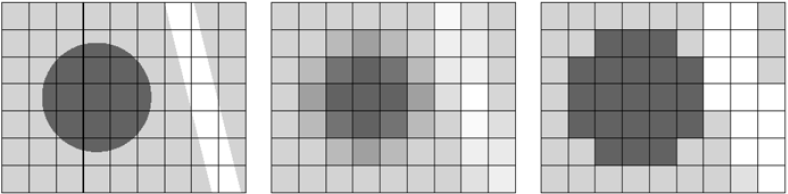
\includegraphics[scale = 0.7]{Content/Pictures/partial.png}
	\caption{Beispiel für Partialvolumenartefakte: Links zeigt einen Tumor, die Mitte das finale Bild und rechts alle Voxel in denen Grauwerte des Tumors verzeichnet wurden \cite{DerDigitaleOperationssaal}}
	\label{fig:partial}
\end{figure}

\subsection{Kosten- Nutzen Verhältnis}

Eine der wichtigen Fragen die noch geklärt werden muss, ist ob ein Hybrider OP-Saal tatsächlich den Mehraufwand an Kosten und Umstrukturierung lohnt. Die benötigte Raumgröße und Ausrüstung führen dazu, dass ein Hybrider OP-Saal in der Anschaffung mehr als doppelt so teuer und in der Wartung fast doppelt so teuer wie ein konventioneller OP-Saal ist \cite{HybridOR}. \\
Gleichzeitig hat sich herausgestellt, dass neue medizinische Technologien meist positiv aufgenommen werden, obwohl ein Mehrwert dieser noch gar nicht bewiesen wurde. Dies und die Digitalisierung des Operationssaals, hat in den letzten Jahren zu erheblichen Steigerung der Gesundheitskosten beigetragen \cite{DerDigitaleOperationssaal}.

%TODO umformulieren, Fragen hab ich ja jetzt entfert
Weil die oben genannten Fragestellungen nicht wirklich beantwortet werden können, soll herausgearbeitet werden, welchen Mehrwert der Hybride OP-Saal tatsächlich bringt. Weil die Vorteile des Hybriden OP-Saals bereits im ersten Kapitel herausgearbeitet wurden, wird hier deshalb nur auf die Kosten und Operationszeit eingegangen.
% auf die Sterblichkeitsrate, Operationszeit und Kosten eingegangen.

Im Anwendungsfall des Bauchaortenaneurysma konnte eine Operationszeiteinsparung von 23,5 Minuten (von 120 auf 96,5 Minuten), mit einem Hybriden OP-Saal gegenüber einem konventionellen mit C-Bogen, erreicht werden. Die Zeiteinsparung führt zusätzlich auch zu einer Kosteneinsparung der Prozesskosten und beträgt 276,17€ weniger pro durchgeführte Operation.
Dieses Ergebnis muss jedoch kritisch betrachtet werden, da die Studie auf Ergebnissen eines konventionellen OPs mit 97 Patienten von 2007 bis 2010 und beim Hybriden mit 50 Patienten von 2012 bis 2015 durchgeführt wurde. Ein positiver Trend ist dennoch sehr wohl zu verzeichnen, da bei den Patienten und dem Operationsteam sehr auf  ähnliche Charakteristika geachtet wurde \cite{HybriderVsKonventioneller}.
Trotzdem können zwei so komplexe Systeme wie hier betrachtet, kaum miteinander verglichen werden. Trotz enormer Ähnlichkeiten wird immer einen gewisser Unterschied zwischen den verglichenen Patienten und Teams bleiben \cite{DerDigitaleOperationssaal}.

Dennoch ist durch die Operationszeiteinsparung im Hybriden OP-Saal eine Refinanzierung möglich \cite{HybriderVsKonventioneller}. Hinzu kommen positive Ergebnisse ohne einen direkten Vergleichswert, wie beispielsweise bei der Tumorentfernung. Bei 14 aus 16 Fällen konnten die Tumore komplett entfernt werden und mögliche auftretende Brain Shifts frühzeitig erkannt werden \cite{BrainShiftInTumorResection}.

Da Studien zum Vergleich zwischen einem Hybriden und Konventionellen Operationssaal zum einen kaum vorliegen und zum anderen schwierig durchzuführen und zu validieren sind, lässt sich die Frage zum tatsächlichen Nutzen sehr schwer beantworten. Hinzu kommt, dass man nicht einfach nur die Todesraten bei bestimmten Krankheitsbildern miteinander vergleichen kann, da diese teilweise sehr gering sind und sehr viele Probanden verglichen werden müssten, was in den meisten Fällen gar nicht möglich ist. Darüber hinaus geht eine verbesserte Überlebensrate nicht immer auch mit einer verbesserten Lebensqualität mit ein \cite{HybriderVsKonventioneller}. \\
Weitere wichtige Faktoren, die einen Einfluss auf den Nutzen haben, sind die gefühlte und tatsächliche Sicherheit von Patienten und Chirurgen. Die psychologische Seite ist jedoch noch viel schwieriger zu bewerten als das tatsächliche objektive Ergebnis \cite{DerDigitaleOperationssaal}.

Trotzdem lässt sich festhalten, dass der Hybride OP-Saal seine Vorteile mit sich bringt. Nicht in allen medizinischen Bereichen wird er einen gleichgroßen Nutzen zur Geltung bringen aber in denjenigen in denen er dies tut, eröffnen sich völlig neue Möglichkeiten zur Operationsdurchführung und somit stellt er die Zukunft des Operationssaals dar \cite{ORofTheFuture}.
%TODO Herausforderungen: auf  Brain Shift, Aortenaneurysma, Tumorentfernung und Herzchirurgie Todesrate wieder drauf eingehen wenn möglich

\subsection{Planung der Räumlichkeiten}

Die Raumplanung eines Hybriden OP-Saals ist ein sehr komplexer Prozess, da er mehreren Fachbereichen gerecht werden muss, die unterschiedliche und teilweise auch sich gegenseitig ausschließende Ansprüche haben. Aus diesem Grund müssen alle fachbereichsübergreifenden Chirurgen aber auch Anästhesisten, Arzthelfer und Techniker in den Planungsprozess miteinbezogen werden.
Gleichzeitig ist durch die erhöhte Anzahl an Mitgliedern (8 bis 20 Personen) im Operationsteam eine Raumgröße von circa 70m² empfehlenswert. Mit Kontroll-, Technik und Vorbereitungsraum müssen dann insgesamt mit circa 150m² gerechnet werden. Je nachdem ob die Geräte und Systeme wie der C-Bogen über eine Decken- oder Bodenbefestigung angebracht werden, müssen diese einem Gewicht von 650 bis 1800kg standhalten. Gleichzeitig dürfen die bildgebenden Systeme, Monitore, Beleuchtungsanlagen und das Personal nicht miteinander Kollidieren (Abb. \ref{fig:roomplanning}). Durch die große Raumgröße und Montage von Geräten an der Decke, wird zusätzlich noch die Einhaltung der Hygienevorschriften erschwert \cite{TechnicalConsiderations}.\\ 
Aus den genannten Gründen muss normalerweise mit einer relativ langen Planungsphase für einen Hybriden OP-Saal gerechnet werden, um allen Ansprüchen einigermaßen gerecht zu werden und einen zukunftsfähigen OP-Saal zu errichten.

\begin{figure} [H]
	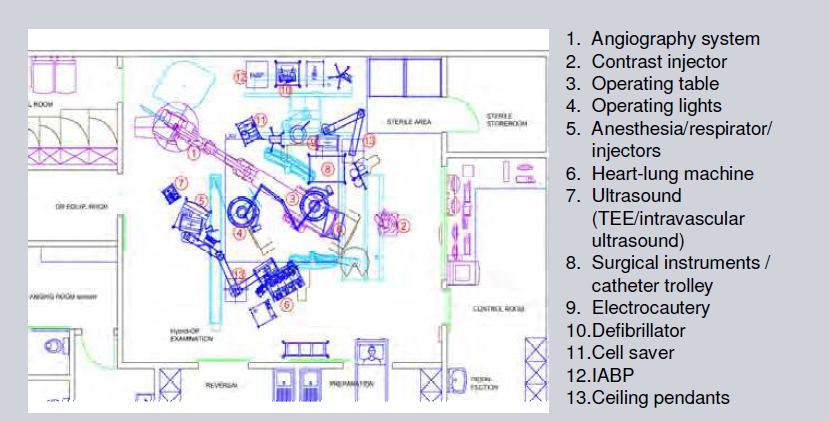
\includegraphics[scale = 0.7]{Content/Pictures/roomplanning.png}
	\caption{Beispielhaftes Layout für die Planung eines Hybriden OP-Saals \cite{HybridOR}}
	\label{fig:roomplanning}
\end{figure}


 






\chapter{\iflanguage{ngerman}{Zukünftige Entwicklung}{Development}}
\label{sec:overview}

%TODO Herausforderungen zukünftige Entwicklung und aktuell drauf eingehen
%TODO Ausblick (deshalb diese Kapitel zum Schluss)

\subsection{Neue Technologien}

\subsection{Forschung}

	
	
	





\bibliography{Bibliography/thesis}


\end{document}
